% Avant de compile to PDF, s'assurer d'être en mode knitr au lieu de Sweave
% Pour ce faire : Global options - Sweave - Weave rnw files with - Knitr.
%
% Thx


%%% SCRIPT PART:





\documentclass{article}\usepackage[]{graphicx}\usepackage[]{color}
%% maxwidth is the original width if it is less than linewidth
%% otherwise use linewidth (to make sure the graphics do not exceed the margin)
\makeatletter
\def\maxwidth{ %
  \ifdim\Gin@nat@width>\linewidth
    \linewidth
  \else
    \Gin@nat@width
  \fi
}
\makeatother

\definecolor{fgcolor}{rgb}{0.345, 0.345, 0.345}
\newcommand{\hlnum}[1]{\textcolor[rgb]{0.686,0.059,0.569}{#1}}%
\newcommand{\hlstr}[1]{\textcolor[rgb]{0.192,0.494,0.8}{#1}}%
\newcommand{\hlcom}[1]{\textcolor[rgb]{0.678,0.584,0.686}{\textit{#1}}}%
\newcommand{\hlopt}[1]{\textcolor[rgb]{0,0,0}{#1}}%
\newcommand{\hlstd}[1]{\textcolor[rgb]{0.345,0.345,0.345}{#1}}%
\newcommand{\hlkwa}[1]{\textcolor[rgb]{0.161,0.373,0.58}{\textbf{#1}}}%
\newcommand{\hlkwb}[1]{\textcolor[rgb]{0.69,0.353,0.396}{#1}}%
\newcommand{\hlkwc}[1]{\textcolor[rgb]{0.333,0.667,0.333}{#1}}%
\newcommand{\hlkwd}[1]{\textcolor[rgb]{0.737,0.353,0.396}{\textbf{#1}}}%
\let\hlipl\hlkwb

\usepackage{framed}
\makeatletter
\newenvironment{kframe}{%
 \def\at@end@of@kframe{}%
 \ifinner\ifhmode%
  \def\at@end@of@kframe{\end{minipage}}%
  \begin{minipage}{\columnwidth}%
 \fi\fi%
 \def\FrameCommand##1{\hskip\@totalleftmargin \hskip-\fboxsep
 \colorbox{shadecolor}{##1}\hskip-\fboxsep
     % There is no \\@totalrightmargin, so:
     \hskip-\linewidth \hskip-\@totalleftmargin \hskip\columnwidth}%
 \MakeFramed {\advance\hsize-\width
   \@totalleftmargin\z@ \linewidth\hsize
   \@setminipage}}%
 {\par\unskip\endMakeFramed%
 \at@end@of@kframe}
\makeatother

\definecolor{shadecolor}{rgb}{.97, .97, .97}
\definecolor{messagecolor}{rgb}{0, 0, 0}
\definecolor{warningcolor}{rgb}{1, 0, 1}
\definecolor{errorcolor}{rgb}{1, 0, 0}
\newenvironment{knitrout}{}{} % an empty environment to be redefined in TeX

\usepackage{alltt}

\usepackage[utf8]{inputenc}
\usepackage{url}
\usepackage[toc,page]{appendix}
\renewcommand{\appendixpagename}{Annexes}
\renewcommand{\appendixtocname}{Annexes}
\renewcommand{\contentsname}{Table des matières}
\IfFileExists{upquote.sty}{\usepackage{upquote}}{}
\begin{document}

\thispagestyle{empty}
\begin{center}

\vspace{3cm}

\textsc{\Large École d'actuariat}\\
\textsc{\Large Université Laval}\\[0.5cm]

\vspace{5cm}

{ \LARGE \bfseries Travail pratique 1  \\ }

\vfill

\Large Guillaume \textsc{Michel}\\
\Large Nathanaël \textsc{Pelchat}\\
\Large Mikael \textsc{Robertson}\\
\Large Olivier \textsc{Turcotte}\\
\vspace{3cm}
{\Large \textsc{Automne} 2018}

\end{center}
\newpage




\section{Sommaire exécutif}
\label{sec:sommaire}


%%Table des matières
\newpage
\tableofcontents
\newpage

\section{Analyse des données} 
\label{sec:analyse}
Pour le moment, j'ai juste foutu tous les graphiques disponibles. Aucune structure.

Voici les variables disponibles afin d'effectuer un modèle prédictif de la perte économique:

\begin{table}[htb]
\caption{Description des variables}
\begin{tabular}{lll}
\hline
\textbf{Variables} & \textbf{Type}        & \textbf{Description}                                         \\ \hline
CASENUM            & Valeur entière       & Numéro d'identification de la réclamation                    \\ \hline
ATTORNEY           & Variable indicatrice & Indique si le réclamant est représenté par un avocat         \\ \hline
CLMSEX             & Variable indicatrice & Indique le sexe du réclamant                                 \\ \hline
MARITAL            & Variable polytomique & Indique le statut marital du réclamant                       \\ \hline
CLMINSUR           & Variable polytomique & Indique si le réclamant est assuré                           \\ \hline
SEATBELT           & Variable polytomique & Indique si le réclamant portait une ceinture de sécurité     \\ \hline
CLMAGE             & Valeur entière       & Âge du réclamant                                             \\ \hline
LOSS               & Valeur continue      & Perte économique totale du réclamant  en milliers de dollars \\ \hline
\end{tabular}
\end{table}

\newpage
\begin{knitrout}
\definecolor{shadecolor}{rgb}{0.969, 0.969, 0.969}\color{fgcolor}
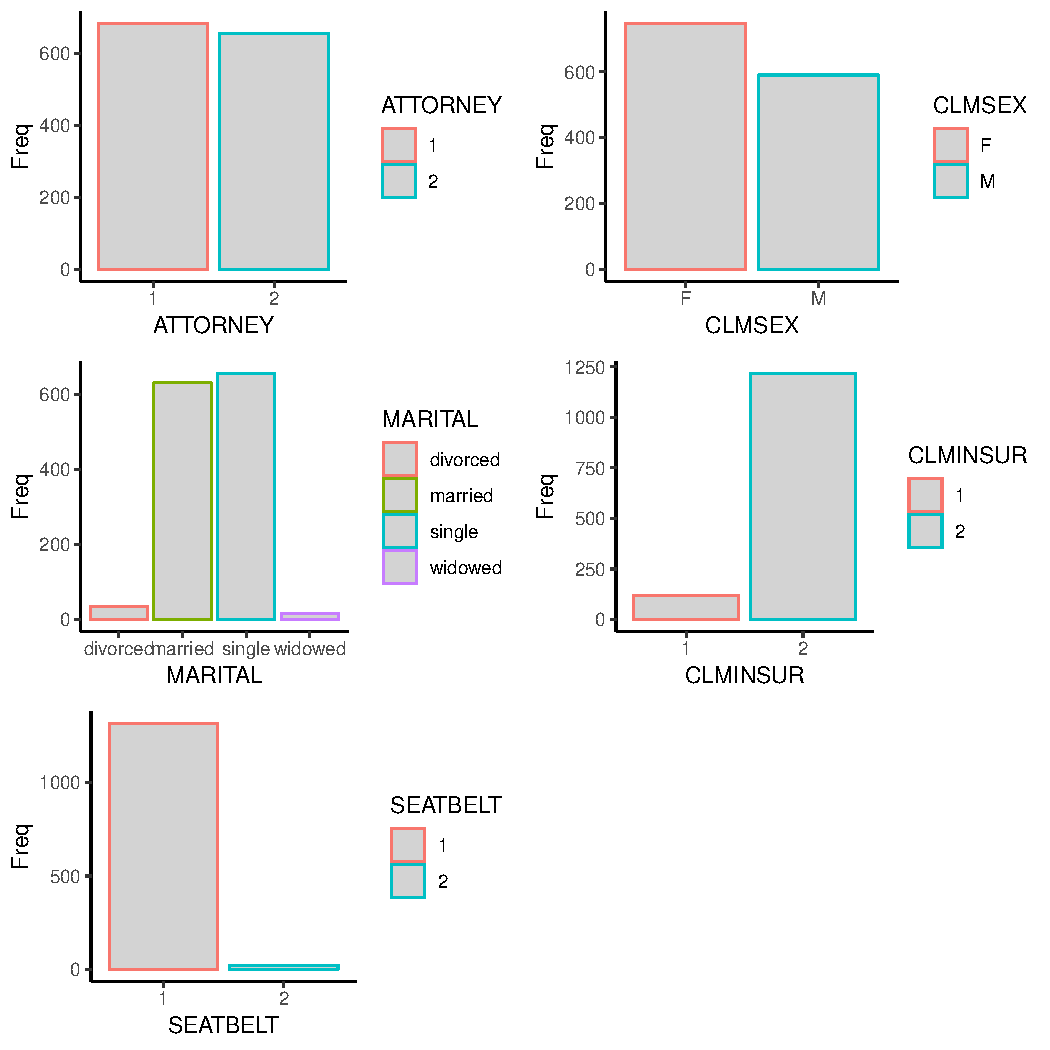
\includegraphics[width=\maxwidth]{figure/unnamed-chunk-2-1} 

\end{knitrout}

\begin{knitrout}
\definecolor{shadecolor}{rgb}{0.969, 0.969, 0.969}\color{fgcolor}\begin{kframe}
\begin{verbatim}
##      CLMAGE            LOSS         
##  Min.   :  0.00   Min.   :   0.005  
##  1st Qu.: 21.00   1st Qu.:   0.640  
##  Median : 33.00   Median :   2.331  
##  Mean   : 33.01   Mean   :   5.965  
##  3rd Qu.: 41.00   3rd Qu.:   3.998  
##  Max.   :610.00   Max.   :1067.697
\end{verbatim}
\end{kframe}
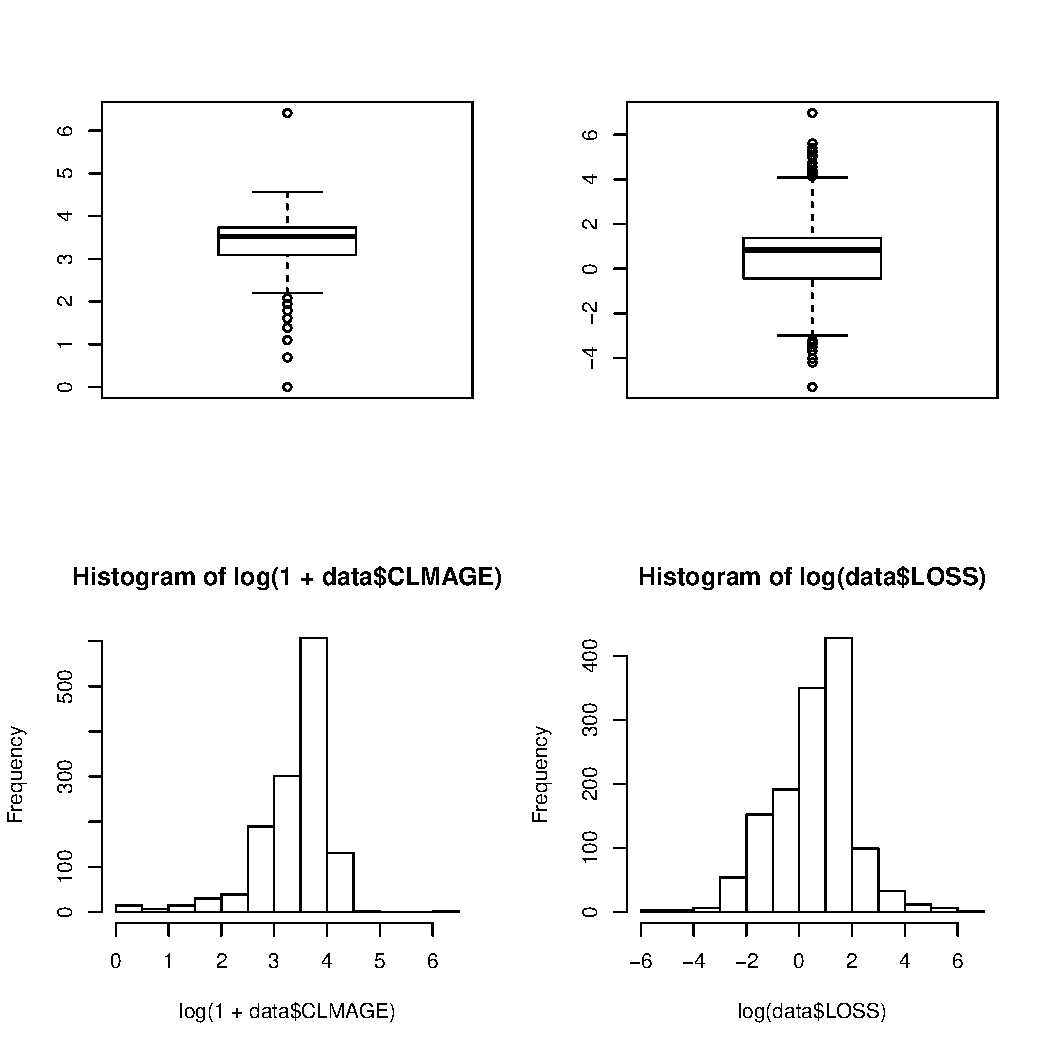
\includegraphics[width=\maxwidth]{figure/unnamed-chunk-3-1} 

\end{knitrout}



\section{Modèle proposé}
\label{sec:modele}

\subsection{Équation}
\label{ssec:equation}

\subsection{Variables qualitatives}
\label{ssec:var_qual}

\subsection{Interactions}
\label{ssec:interaction}

\subsection{Interprétation}
\label{ssec:interpretation}

\subsection{Statistiques}
\label{ssec:stats}

\section{Analyse des résidus}
\label{sec:analyse}

\section{Prévisions}
\label{sec:prev}

\section{Recommendations}


\begin{appendices}
\section{Erreurs de données}

\section{Transformation}

\section{Sélection des variables}
\end{appendices}


\end{document}
